\documentclass[aip, jmp, amsmath, amssymb, reprint, floatfix]{revtex4-1}

\usepackage{graphicx}
\usepackage{dcolumn}
\usepackage{bm}
\usepackage{subfig}
\usepackage{afterpage}	
\usepackage{float}
\usepackage[font={footnotesize}]{caption}


\setlength{\parindent}{4em}
\setlength{\parskip}{0em}
\newcommand{\squeezeup}{\vspace{-4.5mm}}



\begin{figure}
 \centering
 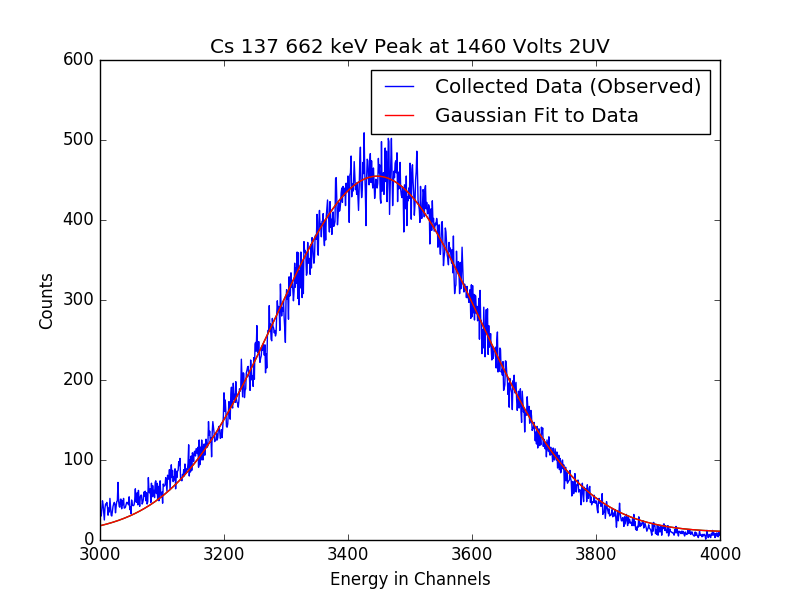
\includegraphics[width=.6\columnwidth]{2UVCsfit.png}
 \caption{Cs 137 UV PMT}
\end{figure}

\begin{figure}
 \centering
 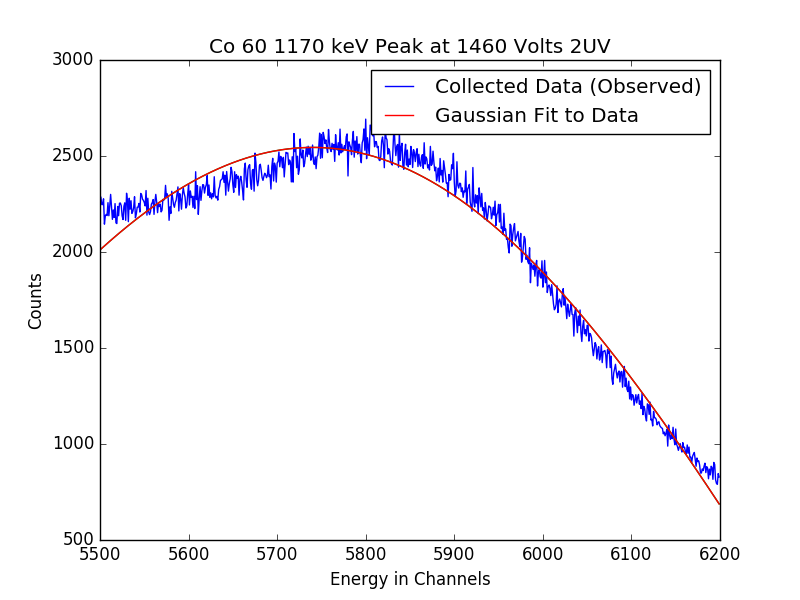
\includegraphics[width=.6\columnwidth]{2UVCo1fit.png}
 \caption{Co 60 Peak 1 UV PMT}
\end{figure}

\begin{figure}
 \centering
 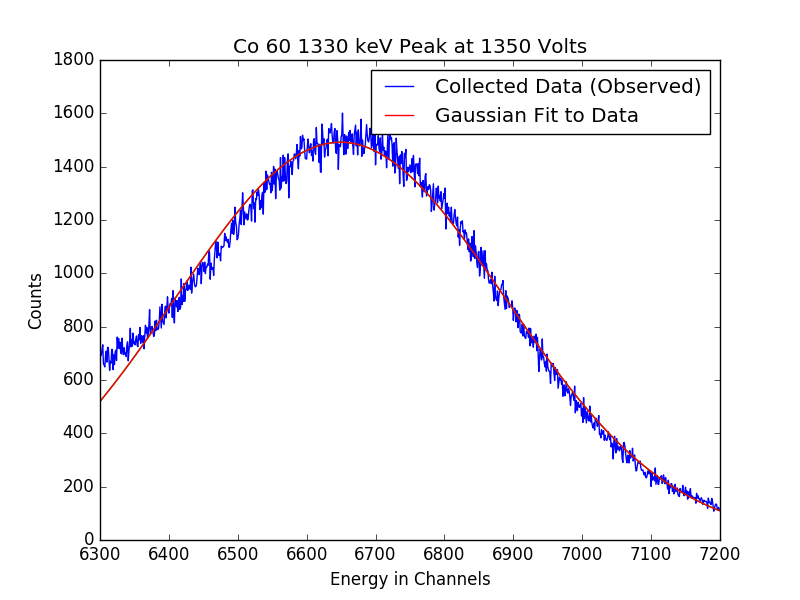
\includegraphics[width=.6\columnwidth]{2UVCo2fit.png}
 \caption{Co 60 Peak 2 UV PMT}
\end{figure}

\begin{figure}
 \centering
 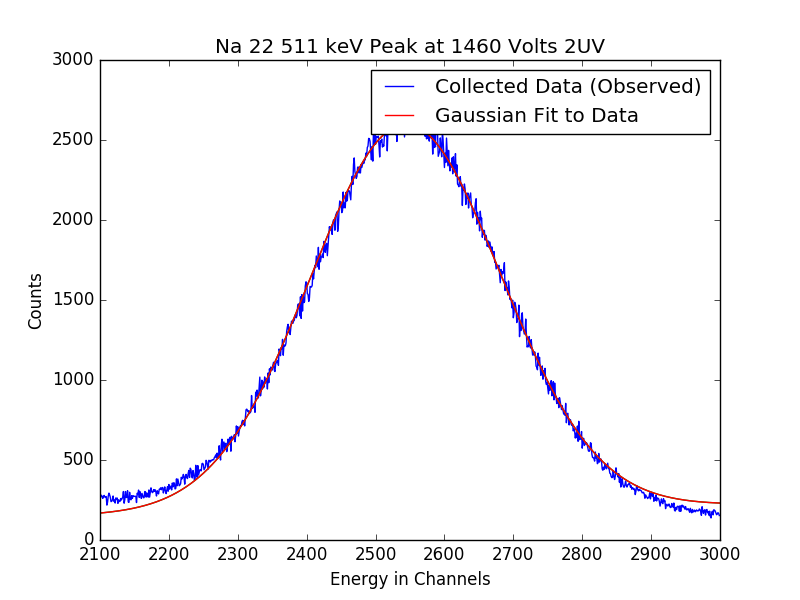
\includegraphics[width=.6\columnwidth]{2UVNa1fit.png}
 \caption{Na 22 Peak 1 UV PMT}
\end{figure}

\begin{figure}
 \centering
 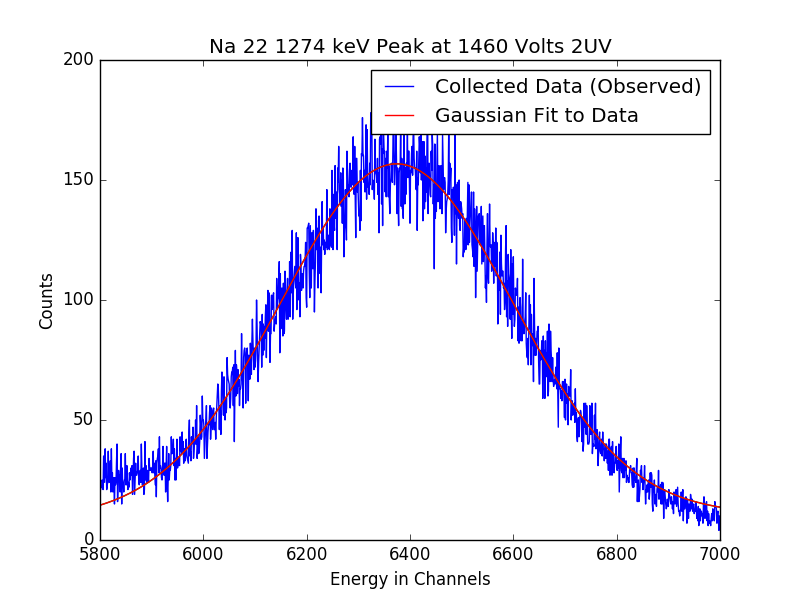
\includegraphics[width=.6\columnwidth]{2UVNa2fit.png}
 \caption{Na 22 Peak 2 UV PMT}
\end{figure}

\begin{figure}
 \centering
 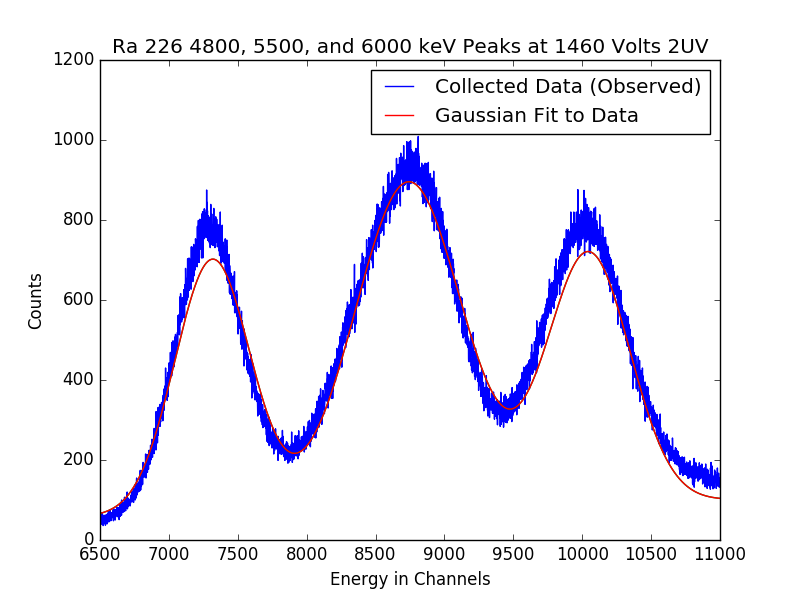
\includegraphics[width=.6\columnwidth]{2UVRa1fit.png}
 \caption{Ra 226 First Three Peaks UV PMT}
\end{figure}

\begin{figure}
 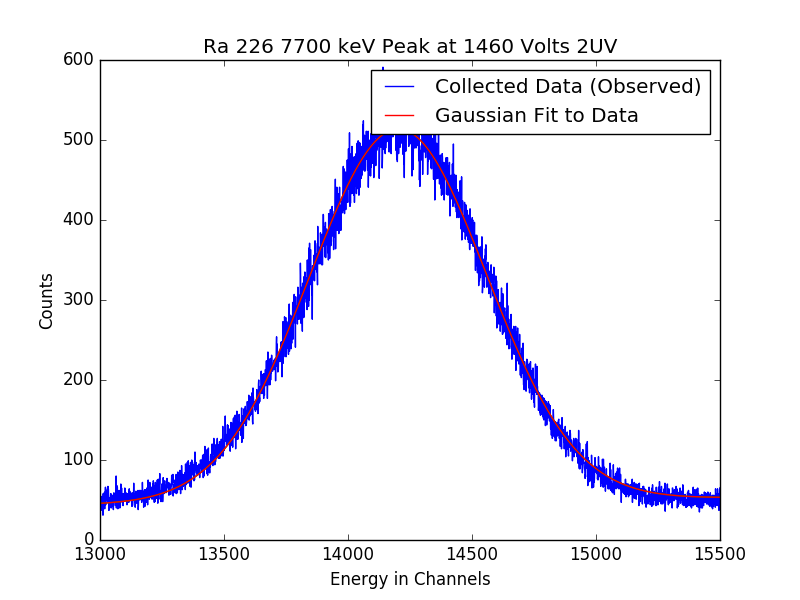
\includegraphics[width=.6\columnwidth]{2UVRa4fit.png}
 \caption{Ra 226 Fourth Peak UV PMT}
\end{figure}

\subsubsection{\label{sec:level3}UV Extended Full Spectrum with Shortpass Filter}

%\begin{figure}
 %\centering
 %\includegraphics[width=.6\columnwidth]{FilAmBefit.png}
 %\caption{AmBe 241 UV PMT with shortpass filter}
%\end{figure}

\begin{figure}
 \centering
 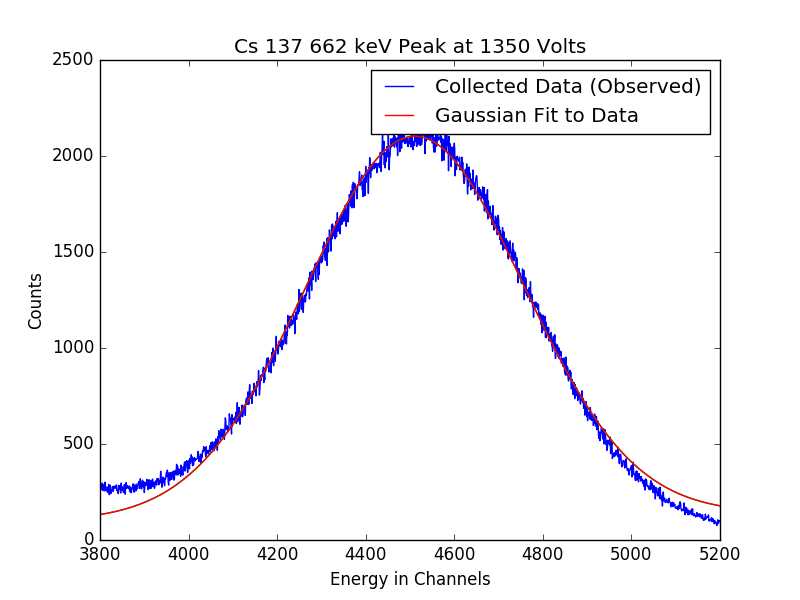
\includegraphics[width=.6\columnwidth]{FilCsfit.png}
 \caption{Cs 137 UV PMT with shortpass filter}
\end{figure}

\begin{figure}
 \centering
 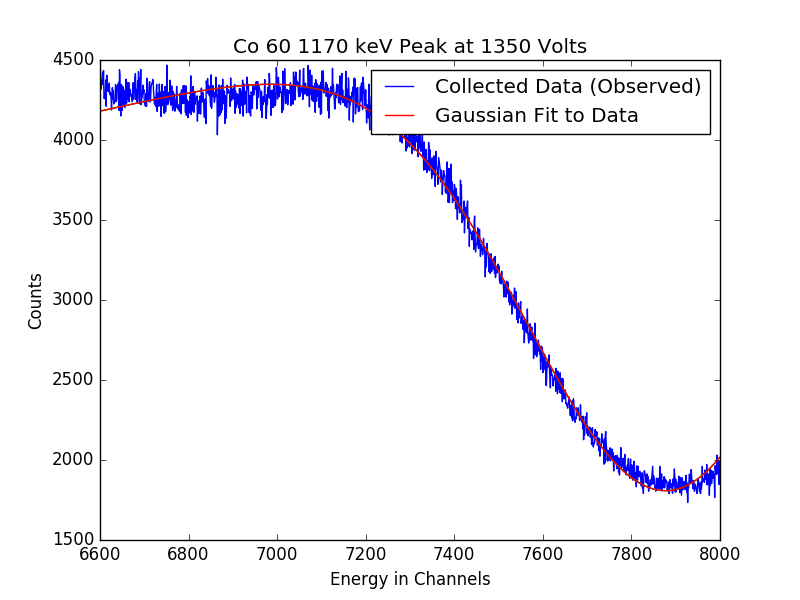
\includegraphics[width=.6\columnwidth]{FilCo1fit.png}
 \caption{Co 60 Peak 1 UV PMT with shortpass filter}
\end{figure}

\begin{figure}
 \centering
 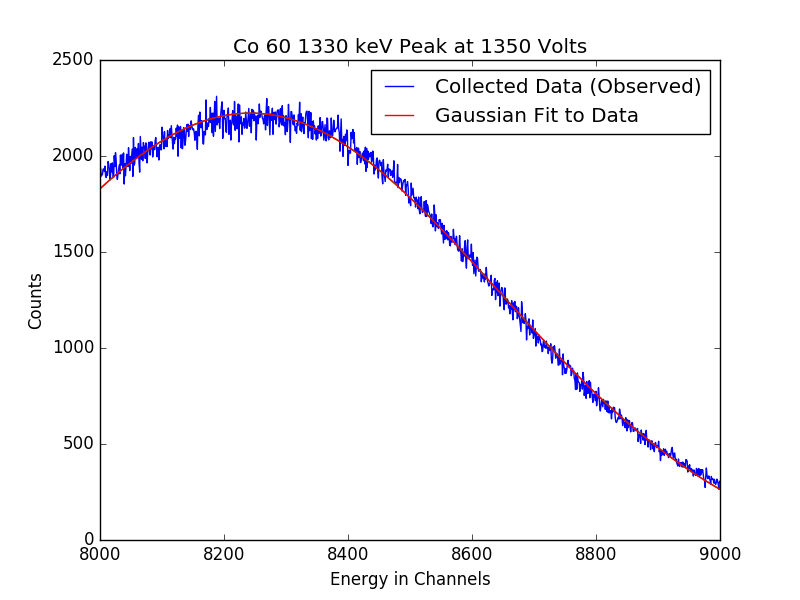
\includegraphics[width=.6\columnwidth]{FilCo2fit.png}
 \caption{Co 60 Peak 2 UV PMT with shortpass filter}
\end{figure}

\begin{figure}
 \centering
 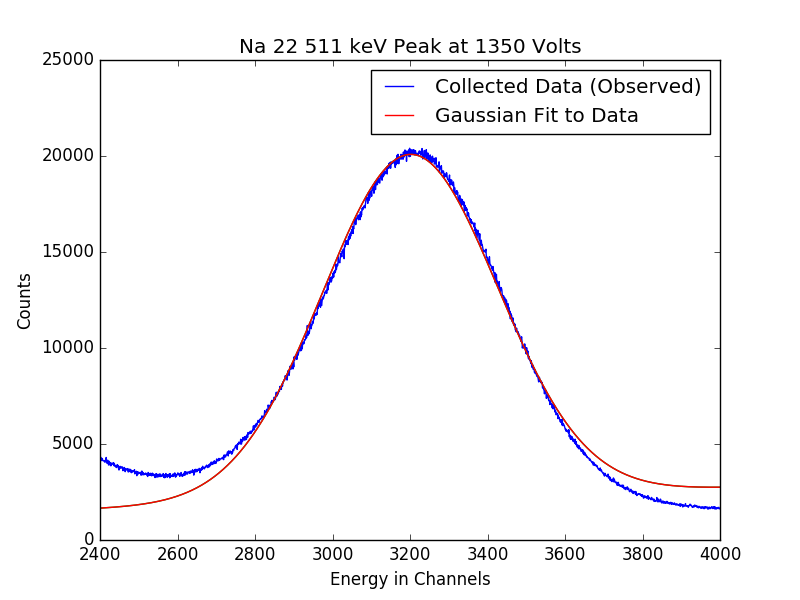
\includegraphics[width=.6\columnwidth]{FilNa1fit.png}
 \caption{Na 22 Peak 1 UV PMT with shortpass filter}
\end{figure}

\begin{figure}
 \centering
 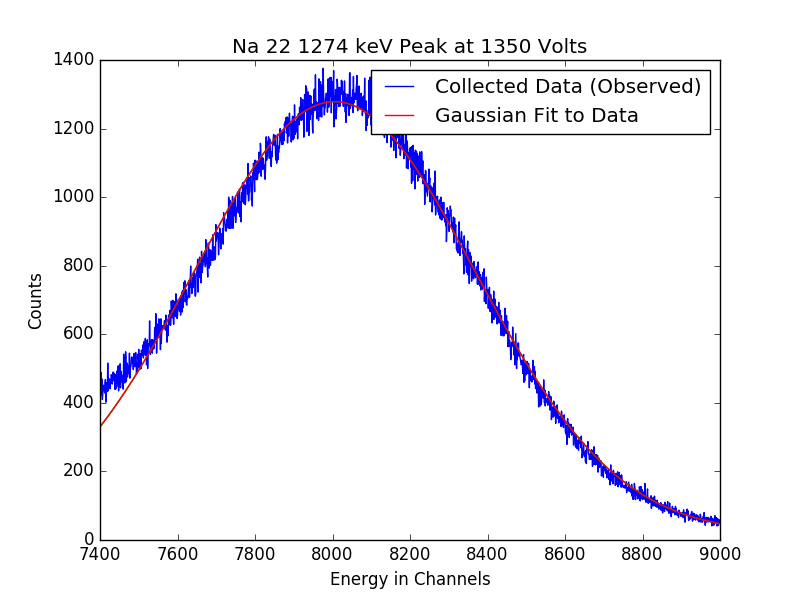
\includegraphics[width=.6\columnwidth]{FilNa2fit.png}
 \caption{Na 22 Peak 2 UV PMT with shortpass filter}
\end{figure}

\begin{figure}
 \centering
 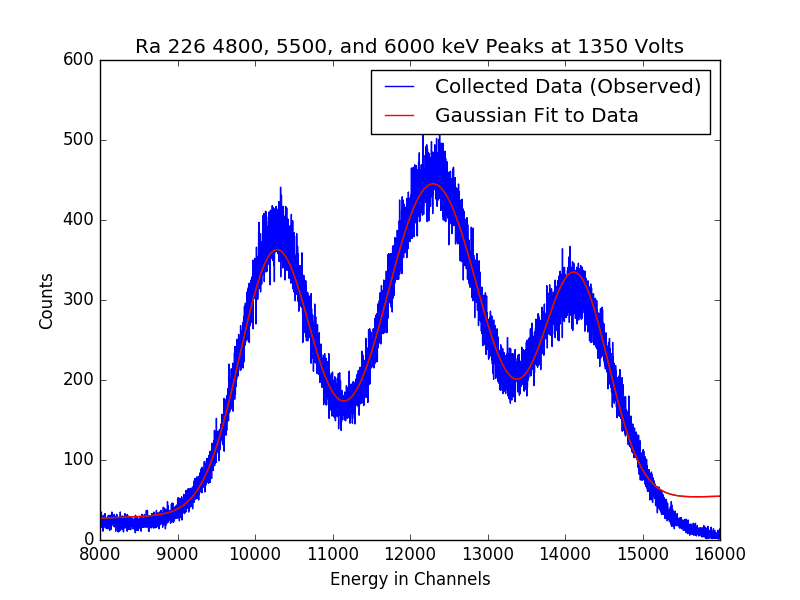
\includegraphics[width=.6\columnwidth]{FilRa1fit.png}
 \caption{Ra 226 First Three Peaks UV PMT with shortpass filter}
\end{figure}

\begin{figure}
 \centering
 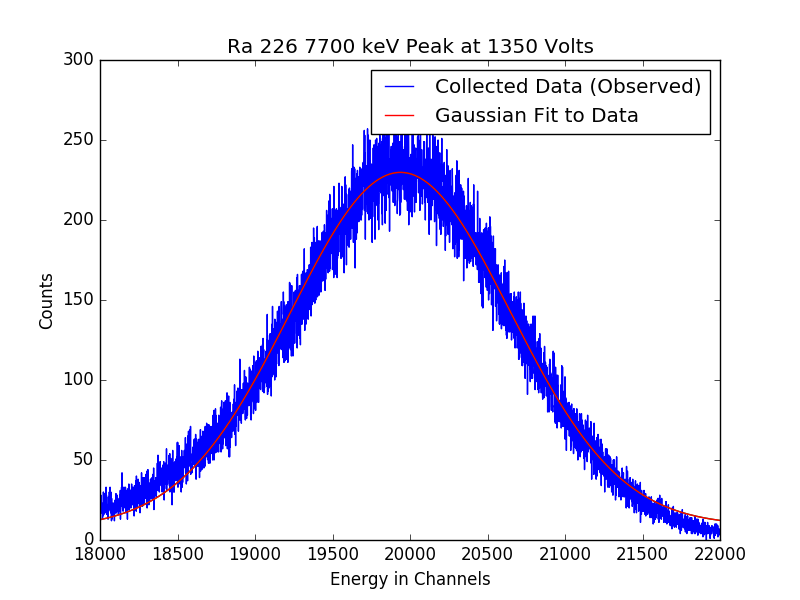
\includegraphics[width=.6\columnwidth]{FilRa4fit.png}
 \caption{Ra 226 Fourth Peak UV PMT with shortpass filter}
\end{figure}

\subsubsection{\label{sec:level3}Solarblind}


\begin{figure}
 \centering
 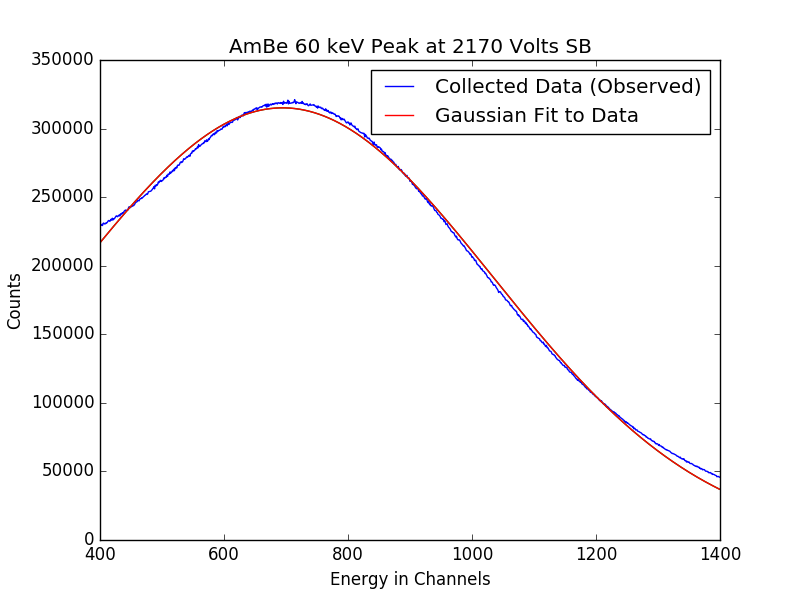
\includegraphics[width=.6\columnwidth]{SBAmBefit.png}
 \caption{AmBe 241 Solarblind PMT}
\end{figure}

\begin{figure}
 \centering
 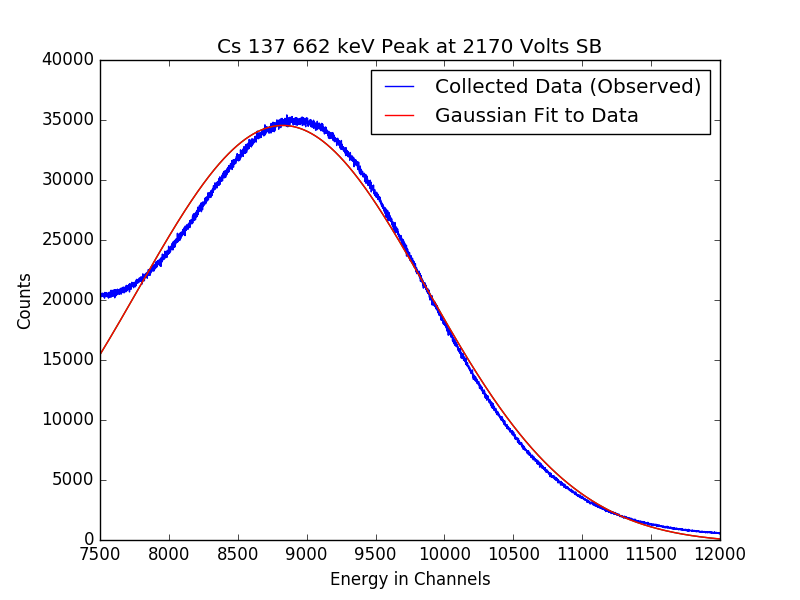
\includegraphics[width=.6\columnwidth]{SBCsfit.png}
 \caption{Cs 137 Solarblind PMT}
\end{figure}

%\begin{figure}
% \centering
% \includegraphics[width=.6\columnwidth]{SBCo1fit.png}
% \caption{Co 60 Peak 1 Solarblind PMT}
%\end{figure}

%\begin{figure}
% \centering
% \includegraphics[width=.6\columnwidth]{SBCo2fit.png}
% \caption{Co 60 Peak 2 Solarblind PMT}
%\end{figure}

\begin{figure}
 \centering
 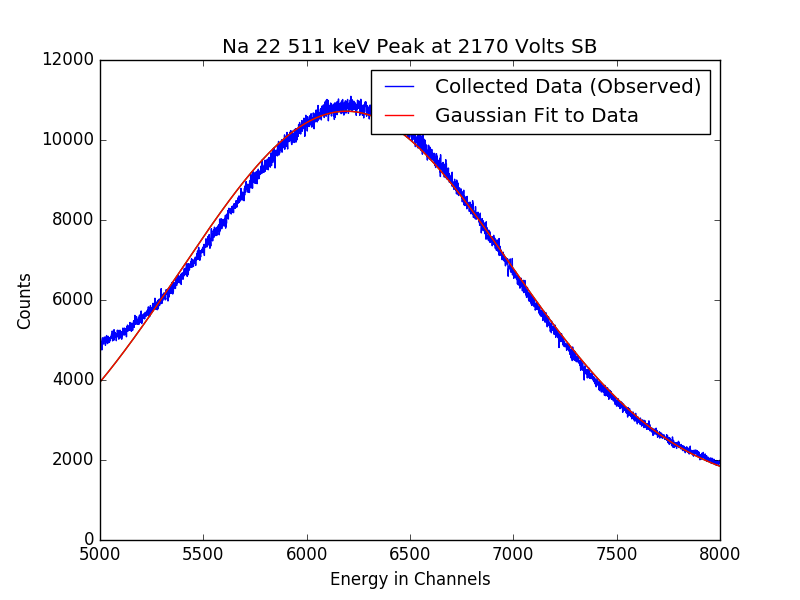
\includegraphics[width=.6\columnwidth]{SBNa1fit.png}
 \caption{Na 22 Peak 1 Solarblind PMT}
\end{figure}

\begin{figure}
 \centering
 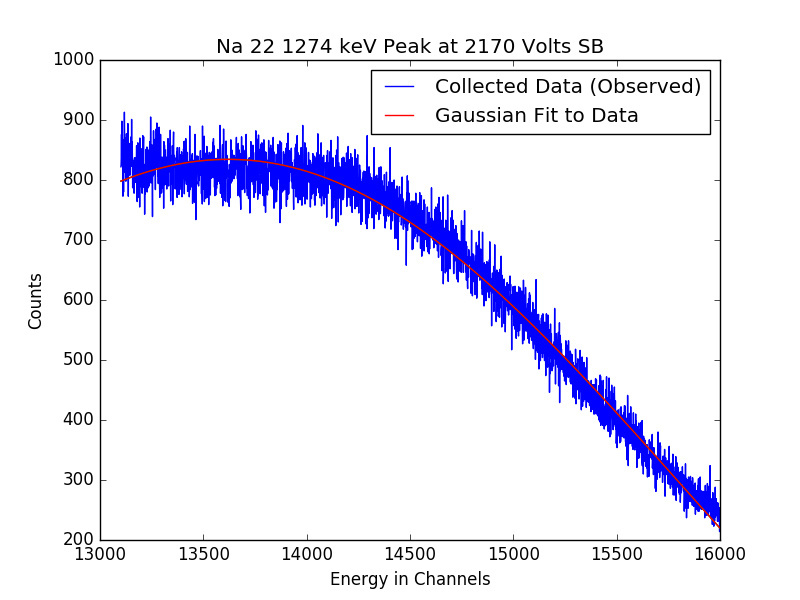
\includegraphics[width=.6\columnwidth]{SBNa2fit.png}
 \caption{Na 22 Peak 2 Solarblind PMT}
\end{figure}

\begin{figure}
 \centering
 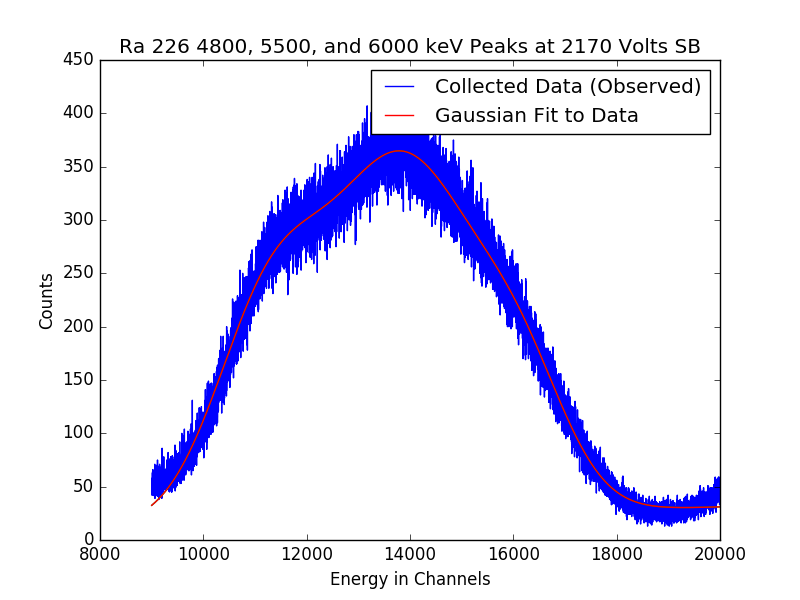
\includegraphics[width=.6\columnwidth]{SBRa1fit.png}
 \caption{Ra 226 First Three Peaks Solarblind PMT}
\end{figure}

\begin{figure}
 \centering
 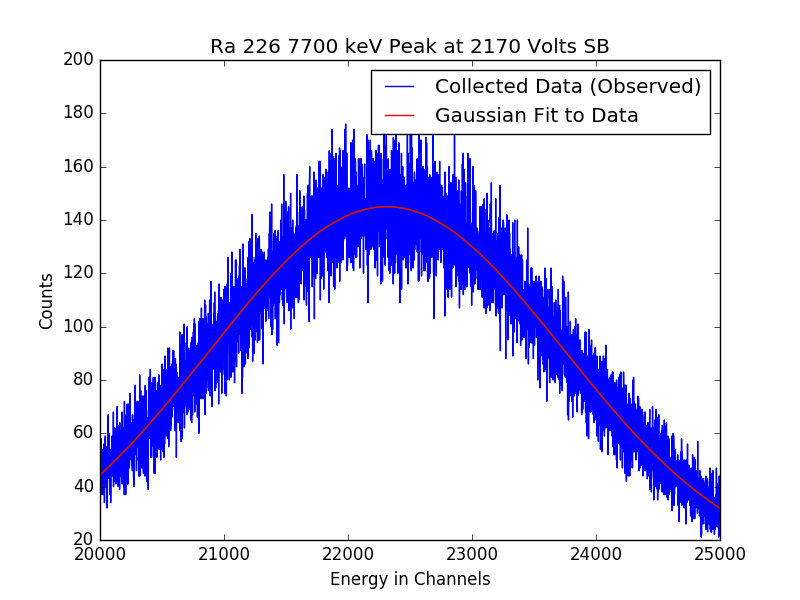
\includegraphics[width=.6\columnwidth]{SBRa4fit.png}
 \caption{Ra 226 Fourth Peak Solarblind PMT}
\end{figure}

\subsection{\label{sec:level2}Quantum Efficiency Spectrum for Each Photomultiplier Tube}

\begin{figure}
 \centering
 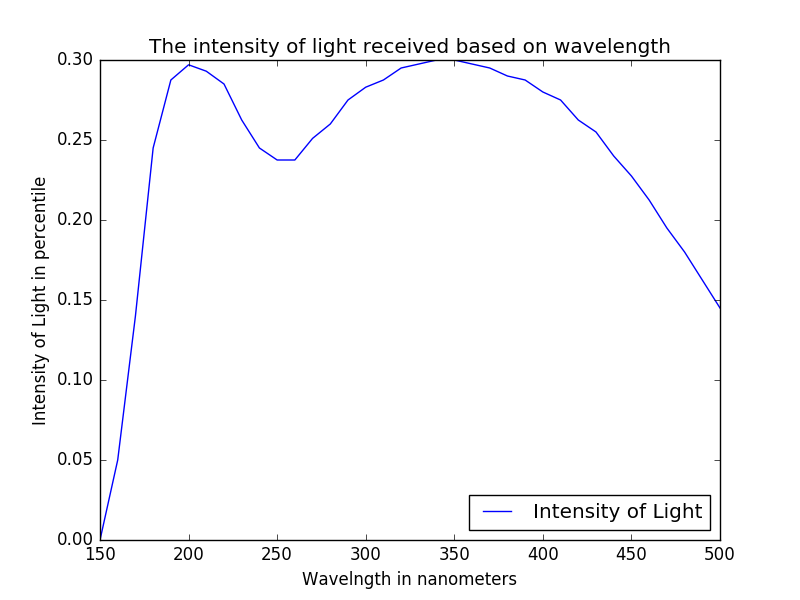
\includegraphics[width=.6\columnwidth]{UVQE.png}
 \caption{UV Extended Full Spectrum PMT QE}
\end{figure}

\begin{figure}
 \centering
 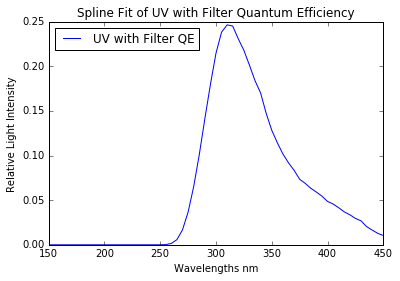
\includegraphics[width=.6\columnwidth]{FilQE.png}
 \caption{UV Extended Full Spectrum with shortpass PMT QE}
\end{figure}

\begin{figure}
 \centering
 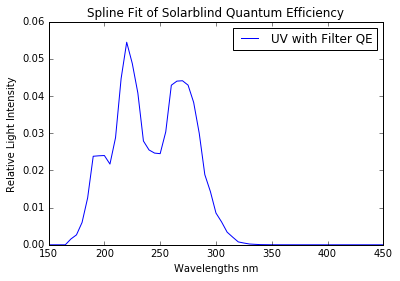
\includegraphics[width=.6\columnwidth]{SBQE.png}
 \caption{Solarblind PMT QE}
\end{figure}


%\subsection{\label{sec:level2}Parameters for each Trial}

%\begin{figure}
 %\centering
 %\includegraphics[width=.6\columnwidth]{parameters.png}
 %\caption{Parameters}
%\end{figure}


%Tables


\begin{table}

\caption{The errors for $\bm{\sigma_s}$}

\label{}

\resizebox{\columnwidth}{!}{%

\begin{tabular}

 \hline

 Component & 4800 & 5500 & 6000 & 7700 \\ \hline

 Slow & 1.36287 & 1.31089 & 1.2333 & 1.10977\\ \hline

 Fast & 0.0290772 & 0.0310162 & 0.0319127 & 0.0313639\\ \hline

\end{tabular}

}

\end{table}

\begin{center}
    \begin{tabular}{ | l | l | l | p{2cm} |}
    \hline
    Component & 4800 & 5500 & 6000 & 7700 \\ \hline

    Slow & 1.36287 & 1.31089 & 1.2333 & 1.10977\\ \hline  

    Fast & 0.0290772 & 0.0310162 & 0.0319127 & 0.0313639\\ \hline
    \hline
    \end{tabular}
\end{center}

\begin{table}[h]
    \begin{tabular}{ | l | l | l | l | p{2cm} |}
    \hline
    Source & AmBe 241 & Cs 137 & Co 60 First Peak & Co 60 Second Peak & Na 22 First Peak \\ \hline

    Energy in keV & 59 &  & 662 & 1170 & 1330 & 511\\ \hline  

    Source & Na 22 Second Peak & Ra 226 First Peak & Ra 226 Second Peak & Ra 226 Third Peak & Ra 226 Fourth Peak \\ \hline

    Energy in keV & 1274 & 4800 & 5500 & 6000 & 7700 \\ \hline
    \hline
    \end{tabular}
  \caption{These values are the previously known energy values of the particles from each radioactive source}
\end{table}


UV with shortpass filter, UV, Solarblind = [6.33012509, 4.984, 12.0694256] 

\begin{table}
    \begin{tabular}{ | l | p{2cm} |}
    \hline
    PMT & Channels to keV\\ \hline

    UV with shortpass filter & 6.33012509\\ \hline  

    UV & 4.984\\ \hline

    Solarblind & 12.0694256\\ \hline
    \hline
    \end{tabular}
    \caption{These values represent the slope of the line from channels (found from the caen output) to keV (from the known values) for each PMT.}
    \label{table:chan_kev}
\end{table}


\setlength{\parskip}{2em}
\noindent
Quenching Factor UV with filter = [2.9762807168446512, 2.8493222446691253, 2.7046015279015254, 2.459904200468519]
\noindent
Quenching Factor UV = [3.269623267619078, 3.1364744649952887, 2.9771822748456365, 2.702319438114875]
\noindent
Quenching Factor Solarblind = [5.155991131280197, 4.789453699584773, 4.475792970019146, 4.166273337999092]

\begin{table}
    \begin{tabular}{ | l | l | l | p{2cm} |}
    \hline
    PMT & 4800 & 5500 & 6000 & 7700\\ \hline

    UV with filter & 2.976 & 2.849 & 2.704 & 2.460\\ \hline  

    UV & 3.269 & 3.136 & 2.977 & 2.702\\ \hline

    Solarblind & 5.155 & 4.789 & 4.475 & 4.166\\ \hline
    \hline
    \end{tabular}
    \caption{These values represent the quenching factor found at each energy level for eahc PMT. These were determined by comparing the expected conversion keV value with the known keV value for each Ra 226 peak}
    \label{table:quench}
\end{table}

\setlength{\parskip}{2em}
\noindent
Fast and Slow Proportions UV with filter = (0.10416262087647044, 0.8958373791235295)
\noindent
Fast and Slow Proportions UV = (0.11286243062670365, 0.8871375693732964)
\noindent
Fast and Slow Proportions Solarblind = (0.5585223540278348, 0.4414776459721652)

\begin{table}
    \begin{tabular}{ | l | l | p{2cm} |}
    \hline
    PMT & Fast Percentage & Slow Percentage\\ \hline

    UV with filter & 0.104 & 0.895\\ \hline  

    UV & 0.112 & 0.887\\ \hline

    Solarblind & 0.558 & 0.441\\ \hline
    \hline
    \end{tabular}
    \caption{These values represent the percentage of light that is from the fast and slow component for each PMT. They are defined as the area under the first two and last two Gaussians of the convolution of the $BaF_2$ emission spectrum and the QE of each PMT}
    \label{table:fastvsslow}
\end{table}

%\begin{eqnarray}
%\ \sigma_s = [1.36287, 1.31089, 1.2333, 1.10977
%\label{eq:twelve}.
%\end{eqnarray}

%\begin{eqnarray}
%\ \sigma_f = [0.0290772, 0.0310162, 0.0319127, 0.0313639]
%\label{eq:thirteen}.
%\end{eqnarray}

\begin{table}[h]
    \begin{tabular}{ | l | l | p{2cm} |}
    \hline
    Component Error & 4800 & 5500 & 6000 & 7700\\ \hline

    Slow Error & 1.362 & 1.310 & 1.233 & 1.109\\ \hline  

    Fast Error & 0.029 & 0.031 & 0.031 & 0.031\\ \hline
    \hline
    \end{tabular}
    \caption{These values represent the error on each fast and slow quenching factor determined from the covariance matrix in the calculation of the point of best intersection.}
    \label{table:fastvsslow}
\end{table}


\begin{figure}
  \centering
    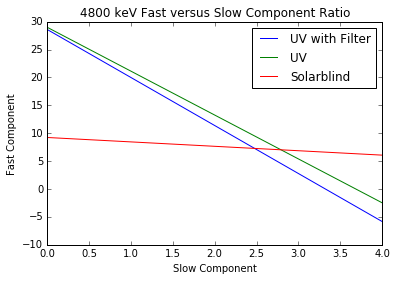
\includegraphics[width=.8\columnwidth]{first.png}
  \caption{4800 Slow versus Fast Componets}
  \label{fig:third}
\end{figure} 

\begin{figure}
  \centering
    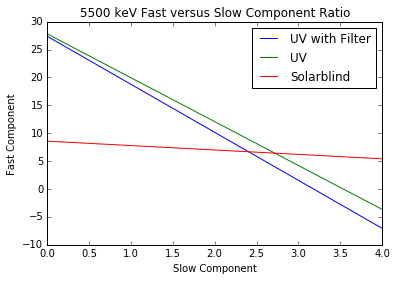
\includegraphics[width=.8\columnwidth]{second.png}
  \caption{5500 Slow versus Fast Componets}
  \label{fig:second}
\end{figure} 

\begin{figure}
  \centering
    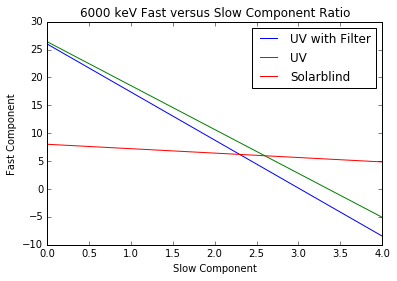
\includegraphics[width=.8\columnwidth]{third.png}
  \caption{6000 Slow versus Fast Componets}
  \label{fig:third}
\end{figure} 

\begin{figure}
  \centering
    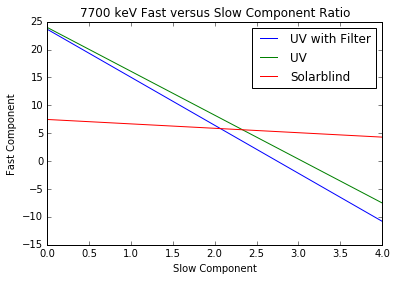
\includegraphics[width=.8\columnwidth]{fourth.png}
  \caption{7700 Slow versus Fast Componets}
  \label{fig:fourth}
\end{figure}
